\documentclass[12pt,letterpaper]{article}
\usepackage[framemethod=tikz]{mdframed}
\usepackage[utf8]{inputenc} %Spanish input
\usepackage[T1]{fontenc} % Use 8-bit encoding that has 256 glyphs
\usepackage[spanish, es-tabla]{babel} % Selecciona el español para palabras introducidas automáticamente
\usepackage{fullpage}
\usepackage[top=2cm, bottom=4.5cm, left=2.5cm, right=2.5cm]{geometry}
\usepackage{lastpage}
\usepackage{enumerate}
\usepackage[inline]{enumitem}
\usepackage{fancyhdr}
\usepackage{xcolor}
\usepackage{listings}
%
\usepackage[sorting=none]{biblatex}
\addbibresource{citas.bib}
%
\usepackage{csquotes}
\usepackage{cellspace}
\setlength{\cellspacetoplimit}{5pt}
\setlength{\cellspacebottomlimit}{5pt}
\usepackage{hhline}
\usepackage{listings}
\usepackage{hyperref}
\usepackage{titletoc,tocloft}
\usepackage{float,subfig}
\setlength{\cftsubsecindent}{2cm}
\setlength{\cftsubsubsecindent}{4cm}
\dottedcontents{section}[1.5em]{}{1.3em}{.6em}
%\usepackage[nodisplayskipstretch]{setspace}
%
\graphicspath{ {./imgs/} } %Drawing the background pic
\usepackage{tikz}
\newcommand{\tikzmark}[1]{\tikz[baseline,remember picture] \coordinate (#1) {};}
\usetikzlibrary{positioning}
\usetikzlibrary{shadows,arrows.meta} % For adding edges label
\usetikzlibrary{calc}
\usepackage{eso-pic}
\AddToShipoutPictureBG{%
    \begin{tikzpicture}[remember picture, overlay]
        \node[opacity=.15, inner sep=0pt]
            at(current page.center){
\includegraphics[scale=1.5]{logo-ugr2}};
    \end{tikzpicture}%
}

% \numberwithin{equation}{section} % Number equations within sections (i.e. 1.1, 1.2, 2.1, 2.2 instead of 1, 2, 3, 4)
% \numberwithin{figure}{section} % Number figures within sections (i.e. 1.1, 1.2, 2.1, 2.2 instead of 1, 2, 3, 4)
% \numberwithin{table}{section} % Number tables within sections (i.e. 1.1, 1.2, 2.1, 2.2 instead of 1, 2, 3, 4)

\hypersetup{%
    colorlinks=true,
    linkcolor=[rgb]{0.2, 0.3, 0.5},
    urlcolor=black,
    citecolor=black,
    linkbordercolor={0 0 1}
}

\renewcommand\lstlistingname{Código:}
\renewcommand\lstlistlistingname{Código:}
\def\lstlistingautorefname{Brian SS.}
%
%
\newcommand{\horrule}[1]{\rule{\linewidth}{#1}} % Create horizontal rule command with 1 argument of height
\definecolor{codegreen}{rgb}{0,0.6,0}
\definecolor{codegray}{rgb}{0.5,0.5,0.5}
\definecolor{codepurple}{rgb}{0.58,0,0.82}
\definecolor{backcolour}{rgb}{0.95,0.95,0.92}
%
\lstset{language=python,basicstyle=\linespread{1.1}\ttfamily\footnotesize,
    xleftmargin=0.0cm, frame=t, framesep=0.15cm, framerule=0pt, tabsize=4,
    showspaces=false, showstringspaces=false,showlines=true,
    keywordstyle=\color{blue}\ttfamily,
    stringstyle=\color{red}\ttfamily,
    commentstyle=\color{gray}\ttfamily,
    morecomment=[l][\color{magenta}]{\#}
}
%
\setlength{\parindent}{0.0in}
\setlength{\parskip}{0.05in}
%
%% Edit these as appropriate
\newcommand\course{Ciencia de Datos e Ingenieria de Computadores}
\newcommand\hwnumber{1}                  % <-- homework number
\newcommand\NetIDa{}           % <-- NetID of person #1
\newcommand\NetIDb{}           % <-- NetID of person #1
%
\pagestyle{fancyplain}
\headheight 35pt
\lhead{\NetIDa}
%\lhead{\NetIDa\\\NetIDb}                 % <-- Comment this line out for problem sets (make sure you are person #1)
\lhead{\textbf{\large Sistemas de visión artificial}}
\rhead{\course \\ \today}
\lfoot{\scriptsize\LaTeX}
\cfoot{\hyperlink{Indice}{Volver al índice}}
\rfoot{\small\thepage}
\headsep 1.5em
%
\renewcommand*\contentsname{Índice}
%
\author{Brian Sena Simons} % Nombre y apellidos
%
\date{\normalsize\today} % Incluye la fecha actual
%
\begin{document}
%
\begin{titlepage}
\begin{figure}[H]
    \vspace{-1.3cm}
    \begin{center}
        
\includegraphics[width=0.75\textwidth]{Etsiit}
    \end{center}
\end{figure}
\vspace{1.3cm}
\centering
\normalfont \normalsize
\textsc{\textbf{Visión por Computador} \\ \vspace{.15cm} Master en Ciencia de Datos e Ingeniería de Computadores \\ \vspace{.15cm} Universidad de Granada} \\ [25pt] % Your university, school and/or department name(s)
    \horrule{0.5pt} \\[0.4cm] % Thin top horizontal rule
    \huge Sistemas de visión artificial\\ % The assignment title
    \horrule{2pt} \\[0.5cm] % Thick bottom horizontal rule

\begin{minipage}{0.4\textwidth}
    \begin{flushleft}\large
        \emph{Autor:} \\
         ----------------------- \\
        \vspace{.15cm}
        Brian Sena Simons. \\

    \end{flushleft}
\end{minipage}
\begin{minipage}{0.4\textwidth}
    \vspace{-2.2cm}
     \begin{flushright}\large
    \end{flushright}
\end{minipage}
\end{titlepage}


\hypertarget{Indice}{}
\tableofcontents
\newpage
\section{Historia de los sistemas de visión}
El estudio y modelado de la visión humana en sistemas inteligentes comenzó a finales de los años 50 con la investigación de Hubel y Wiesel~\cite{CatVisualCortex}, 
quienes analizaron el córtex visual de los gatos. Este trabajo proporcionó avances fundamentales en la comprensión del procesamiento visual, 
evidenciando cómo diferentes áreas del córtex se activan según parámetros como la intensidad lumínica, el ángulo de incidencia, el movimiento y otros factores. 
Los investigadores identificaron tres tipos jerárquicos de células: simples, complejas e hipercomplejas, cada una sintetizando y enriqueciendo la información 
procesada por la anterior. A partir de estas bases, Larry Roberts~\cite{LarryRoberts} realizó una de las primeras tesis doctorales en inteligencia artificial aplicada a la visión artificial. 
Inspirándose en los hallazgos de Hubel y Wiesel~\cite{CatVisualCortex}, propuso métodos para detectar esquinas y puntos de interés, considerando las esquinas como elementos 
cruciales para el reconocimiento y procesamiento de imágenes.

En 1966, se lanzó el ambicioso ``Summer Vision Project''~\cite{SummerVisionProject}, un intento por modelar completamente el sistema visual humano con la participación de solo cinco estudiantes de grado. 
Aunque no logró alcanzar su objetivo, sentó importantes precedentes para futuras investigaciones.  En 1970, David Marr~\cite{DavidMar} propuso un enfoque teórico basado en etapas de procesamiento 
visual, consolidando las ideas previas de Hubel y Wiesel. Su modelo abarcaba aspectos como la detección de esquinas, la estimación de profundidad, la identificación de discontinuidades y 
la construcción de representaciones jerárquicas y volumétricas. Durante esa década, el interés en el reconocimiento de objetos y la segmentación de imágenes 
mediante sistemas inteligentes aumentó significativamente~\cite{PictorialStructures}. Sin embargo, las limitaciones tecnológicas del hardware de la época dificultaban el procesamiento eficiente de imágenes.

Fue en los años 80 cuando surgieron avances clave, como el algoritmo de detección de bordes de Canny~\cite{Canny}, 
que mejoró notablemente la precisión en la identificación de contornos relevantes. 
En la década de 1990, se realizaron avances significativos en el reconocimiento visual mediante la agrupación de elementos dentro de una imagen, 
destacándose el trabajo sobre cortes normalizados~\cite{NormalizedCuts}. 
Esta técnica permitió segmentar imágenes identificando regiones homogéneas, mejorando la eficacia del reconocimiento de patrones complejos.

En 2001, se publicó un artículo clave sobre detección de rostros desarrollado por Viola y Jones~\cite{ViolaAndJones}. Este método revolucionario introdujo el uso de un árbol de decisión que aprendía características específicas para identificar rostros en imágenes, combinando características simples con un clasificador en cascada. 
Fue un hito en la eficiencia de la detección de objetos en tiempo real.
En cuanto a retos visuales, en ese mismo año surgió el \textit{PASCAL Visual Object Challenge}~\cite{PascalVisualObjectChallenge}, 
una competición que proponía problemas de clasificación y detección de objetos en un conjunto de datos compuesto por miles de imágenes cuidadosamente etiquetadas. 
Este desafío incentivó el desarrollo de algoritmos de visión cada vez más robustos y precisos, marcando un antes y un después en la investigación del campo.
Con ello, llegaron en el año 2004 técnicas importantes como SIFT (\textit{Scale-Invariant Feature Transform})\cite{SIFT}, que permitía extraer puntos de interés robustos a variaciones en las imágenes.
En paralelo, en 2005 se introdujeron los histogramas de gradiente orientado (HOG)~\cite{Dalal2005}, 
una técnica que extraía características visuales mediante operaciones convolucionales y que, combinada con máquinas de soporte vectorial (SVM)~\cite{SVM}, mejoró notablemente la clasificación de imágenes.

Un avance fundamental llegó con \textit{ImageNet}~\cite{ImageNet}, el conjunto de datos más grande de su época, que incluía 1,000 categorías y más de un millón de imágenes etiquetadas por colaboradores mediante sistemas de pago por tarea. Este recurso se convirtió en el estándar de referencia para las competencias de visión artificial, permitiendo evaluar y comparar modelos de clasificación a gran escala.
Este hecho facilitó el siguiente gran salto que ocurrió en 2012, cuando Krizhevsky et al.~\cite{AlexNet} introdujeron \textit{AlexNet}, la primera red neuronal convolucional profunda (CNN) que mostró un rendimiento espectacular en ImageNet (véase Figura~\ref{fig:ImageNetProgress}). 
Inspirada en el perceptrón~\cite{Perceptron}, uno de los primeros algoritmos de aprendizaje, \textit{AlexNet} logró una clasificación precisa gracias a su capacidad 
para aprender características complejas directamente de los datos. Esta red fue implementada en hardware gráfico (GPU), acelerando el entrenamiento de grandes volúmenes de imágenes. 
Su éxito abrió las puertas a la era del aprendizaje profundo, revolucionando el campo de la visión por computadora.

\begin{figure}
\begin{center}
    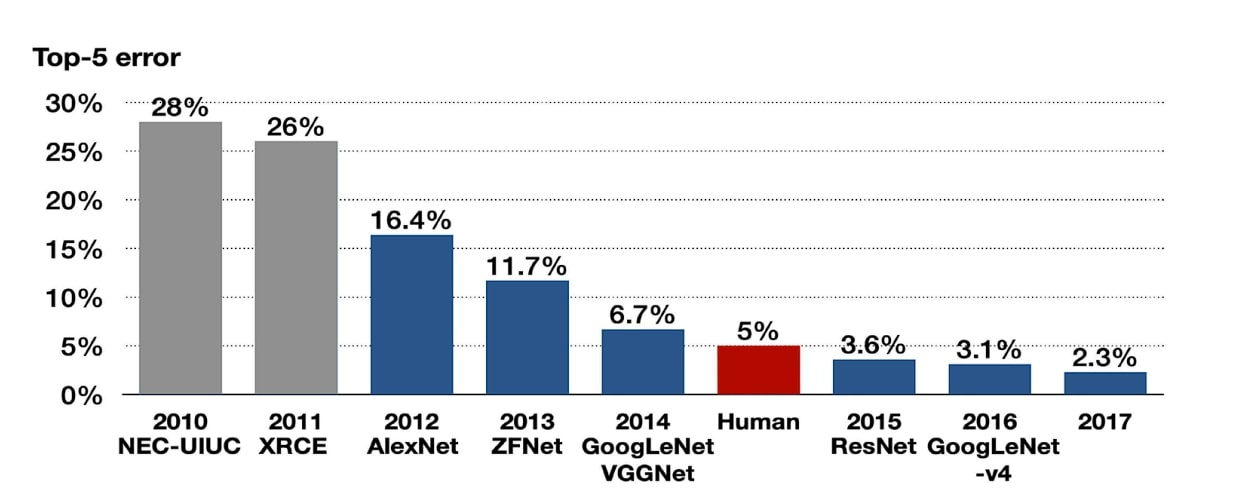
\includegraphics[width=0.5\textwidth]{ImageNetProgress.jpg}
\end{center}
\caption{Observamos el avance en el rendimiento de los sistemas de visión con el tiempo sobre el conjunto ImageNet~\cite{ImageNet}, sacado de ~\cite{ImageNetProgress}.}
\label{fig:ImageNetProgress}
\end{figure}


Para entender este gran salto, tenemos que volver un poco en el tiempo.
Inspirándose en los estudios de Hubel y Wiesel sobre la organización jerárquica del córtex visual~\cite{CatVisualCortex}, en 1980 Fukushima desarrolló el Neocognitron~\cite{Neocognitron}. 
Este modelo introdujo una arquitectura que combinaba células simples (operaciones de convolución) y complejas (operaciones de síntesis o \textit{pooling}), 
sentando las bases de las redes neuronales convolucionales modernas. Sin embargo, el Neocognitron no disponía de un algoritmo eficiente para ajustar sus parámetros, lo que limitaba su aplicabilidad práctica.
El avance crucial llegó en 1986 con la introducción del algoritmo de retropropagación del error (\textit{backpropagation}) por Rumelhart, Hinton y Williams~\cite{Backprop}. 
Este método permitió entrenar redes neuronales de múltiples capas de manera eficiente, allanando el camino para el interés en las redes profundas.
En 1998, LeCun et al.~\cite{LeNet} presentaron \textit{LeNet-5}, una red neuronal convolucional que integraba la retropropagación en una arquitectura similar al \textit{Neocognitron}. 
Esta red demostró su efectividad en la detección de dígitos escritos a mano y fue uno de los primeros modelos en convertirse en un producto comercial, 
utilizado por bancos para el reconocimiento automático de cheques. El desarrollo de estas técnicas de entrenamiento eficientes y la consolidación de arquitecturas 
convolucionales marcaron el inicio de una nueva era para las redes neuronales, con aplicaciones prácticas que continuarían expandiéndose en las décadas siguientes, 
como el gran salto de \textit{AlexNet}~\cite{AlexNet}.

Durante la década de 2000, comenzó una tendencia hacia el entrenamiento de redes neuronales, 
especialmente convolucionales, cada vez más profundas y anchas, dando lugar al concepto de aprendizaje profundo~\cite{Hinton2006,Bengio2007,Lee2009,Glorot2010}, un punto de inflexión en visión por computador. 
Desde entonces, las redes profundas se aplicaron ampliamente en tareas como clasificación de imágenes, recuperación de información visual, detección y segmentación de objetos~\cite{Sun2015,Fabaret2012}, clasificación de vídeos~\cite{Simonyan2014}, reconocimiento de poses~\cite{Toshev2014}, videojuegos~\cite{Guo2015}, imágenes médicas~\cite{Levy2016}, astronomía~\cite{Dieleman2014}, generación de imágenes~\cite{Mordvinsev2015, Gatys2016}, 
y creación de leyendas~\cite{Vinyals2015, Karpathy2015}.

Tras AlexNet, surgieron modelos clave como GoogleNet~\cite{GoogleNet} e Inception~\cite{Inception}. 
Este último destacaba por extraer características a múltiples escalas de forma paralela y fusionarlas en un único mapa multiescala. 
Luego, VGG~\cite{VGG} exploró el efecto de los tamaños de kernels, mostrando que aplicar tres veces un kernel de 3x3 equivale a uno de 7x7, pero con menos parámetros, optimizando así el modelo.
Dos avances cruciales potenciaron aún más la profundidad de las redes convolucionales: el \textit{batch normalization} y los \textit{skip connections}. La primera resolvía el problema del cambio constante en 
la distribución de los datos de entrada durante el entrenamiento, mientras que la segunda mitigaba el desvanecimiento del gradiente permitiendo que este se propagara sin saturarse 
mediante conexiones residuales (véase Figura~\ref{fig:InceptionV3}).
Este progreso no habría sido posible sin el desarrollo paralelo de hardware más potente, 
que facilitó la computación masiva requerida por estos algoritmos complejos, impulsando la evolución de los sistemas de visión artificial (véase Figura~\ref{fig:FlopsPerDollar}).


\begin{figure}[!ht]
\begin{center}
    \includegraphics[width=0.5\textwidth]{InceptionV3}
\end{center}
\caption{Observamos la arquitectura de \textit{InceptionV3}~\cite{InceptionV3}, donde podemos observar una multitud de técnicas avanzadas como el crecimiento en anchura y profundidad, conexiones residuales, capas de normalización y predicción multi-cabeza.}
\label{fig:InceptionV3}
\end{figure}


\begin{figure}[!ht]
\begin{center}
    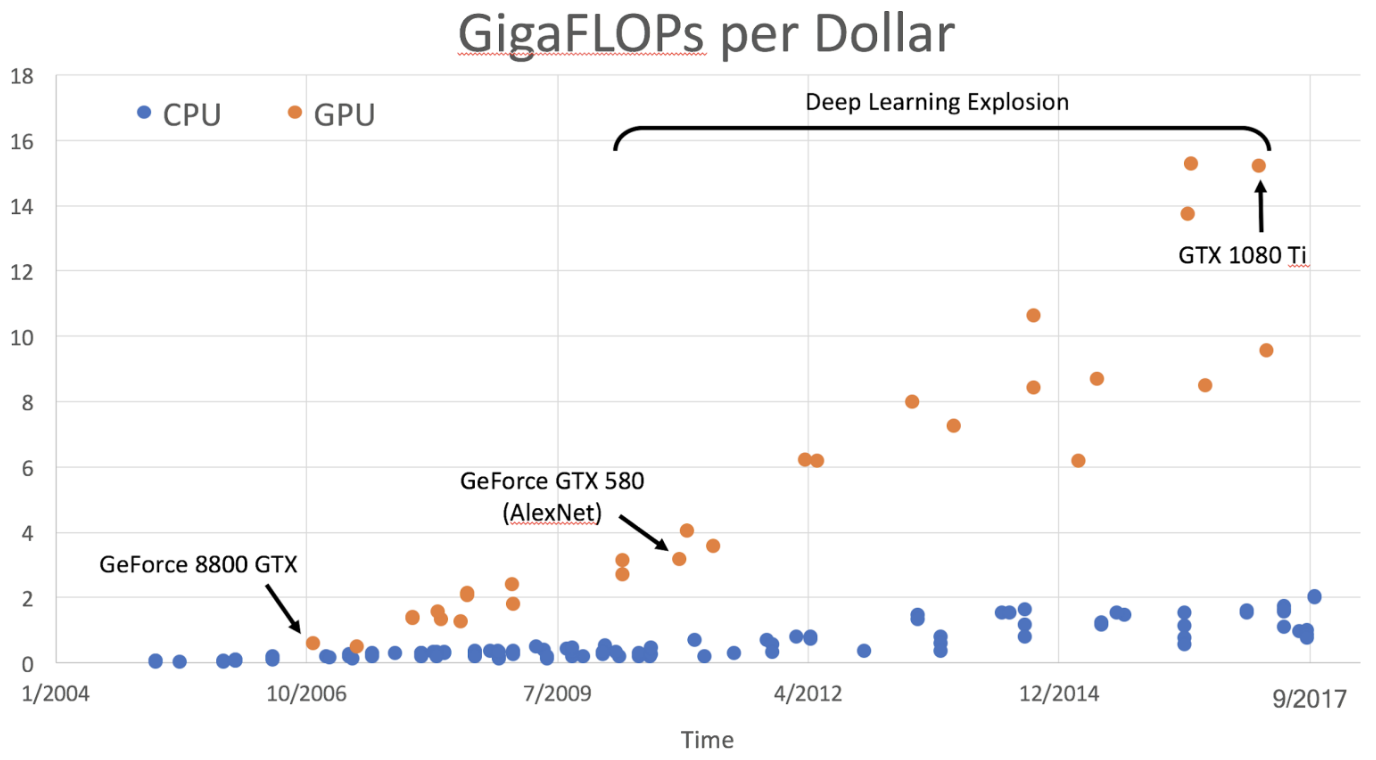
\includegraphics[width=0.5\textwidth]{FlopsPerDollar}
\end{center}
\caption{Observamos el avance en la capacidad de cómputo del hardware, donde se marca la llegada de \textit{AlexNet}~\cite{AlexNet}, sacada de~\cite{Lecture09}.}
\label{fig:FlopsPerDollar}
\end{figure}

Durante los años 2020, los avances más significativos en visión por computador se dieron con la introducción de arquitecturas basadas en Transformers. 
En particular, Vision Transformer (ViT)~\cite{VIT} revolucionó el paradigma al procesar imágenes mediante la extracción de 
parches regulares de tamaño 16x16 que se codifican con vectores posicionales y se introducen en una matriz de atención. 
Esta estrategia permite capturar tanto relaciones locales como globales en las imágenes, de forma muy escalable y superando alguna de las limitaciones 
de las convoluciones tradicionales en redes neuronales. En 2022, ConvNeXt~\cite{ConvNext} apareció como una evolución híbrida que combinó lo mejor de ambos mundos: la eficiencia de los métodos convolucionales y la flexibilidad de los transformers. 
Inspirándose en la arquitectura de los \textit{transformers}, ConvNeXt busca aplicar decisiones de diseño de dichas arquitecturas al cómputo con convoluciones (véase Figura~\ref{fig:ConvNext}). 

\begin{figure}[!ht]
\begin{center}
    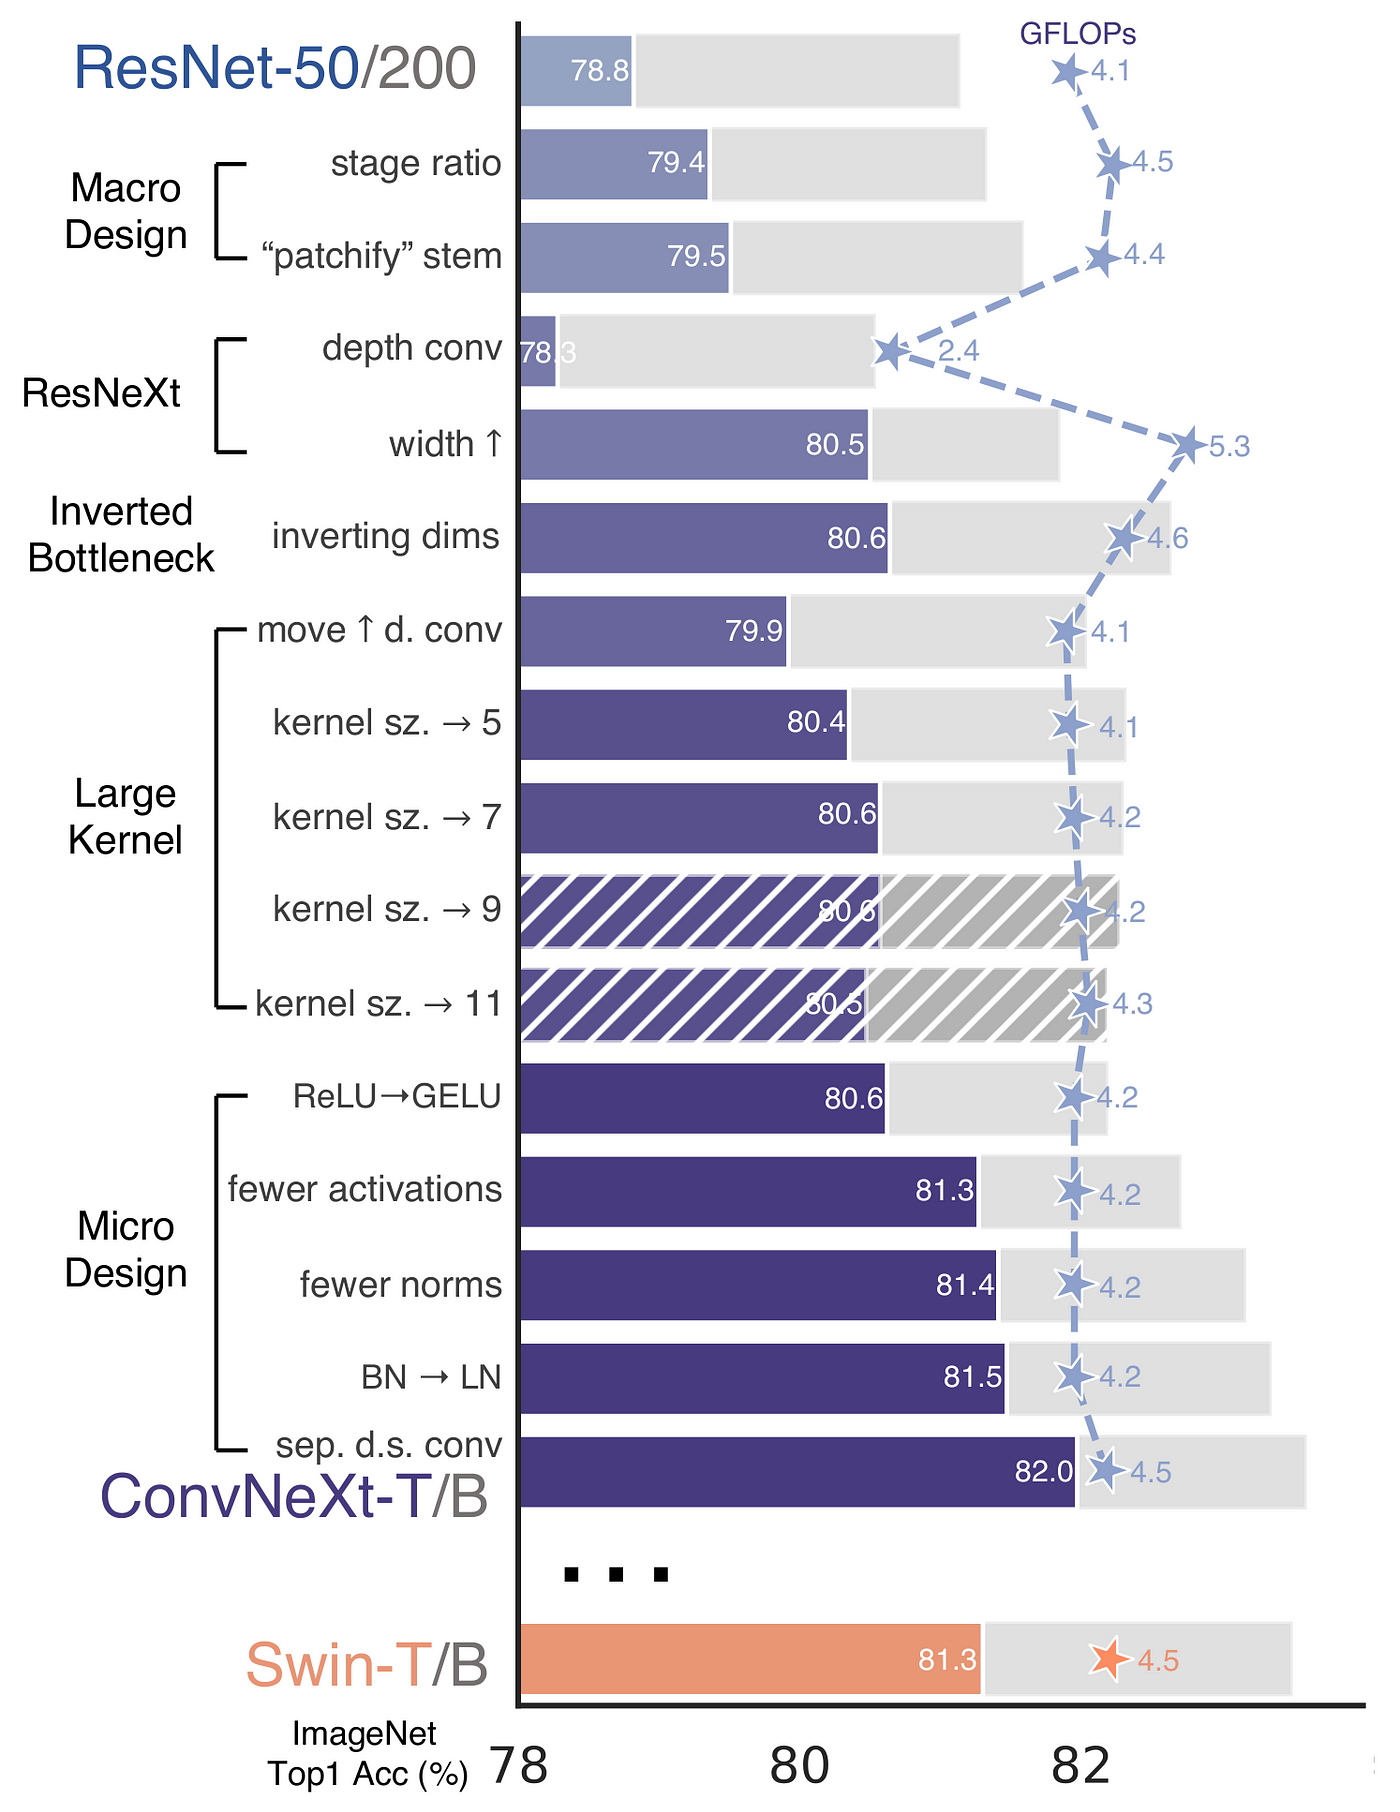
\includegraphics[width=0.45\textwidth]{ConvNext.png}
\end{center}
\caption{Observamos todas las decisiones de arquitectura aplicadas sobre una red convolucional básica, como ResNet~\cite{ResNet}, para obtener una red convolucional con comportamiento similar a los \textit{transformers} (sacada de~\cite{ConvNext}).}
\label{fig:ConvNext}
\end{figure}

\section{Single View Metrology in the wild}
La metrología de vista única tiene una multitud de aplicaciones, desde reconstrucciones en arquitectura, investigación forense y estudio histórico del arte~\cite{SingleViewMetrologyApplications}.
La reconstrucción 3D de imágenes es un problema fundamental de la visión por computador. Pese a los avances, la mayoría de los trabajos reconstruyen las imágenes a escalas desconocidas. Esta ambigüedad es inherente a 
la naturaleza proyectiva de las imágenes y para resolverlo se necesita información adicional. 
En el artículo~\cite{SingleViewMetrology} proponen un método de reconstrucción para escenas ``no controladas'' (cualquier escena) compuesta de objetos de tamaños desconocidos.
Para ello, realizan una calibración geométrica de la cámara, recuperando la orientación de la misma (o, alternativamente, el horizonte en la imagen), el campo de visión y la altura absoluta de la cámara desde el suelo.
Con estos parámetros, es posible convertir cualquier medición 2D en el espacio de la imagen a mediciones 3D (véase Figura~\ref{fig:ExampleObjectInsertion}).

Para resolver este problema se debe calibrar la cámara, los parámetros intrínsecos y extrínsecos. Para lo primero, 
se suele utilizar razonamiento explícito o grandes conjuntos de datos anotados. Para lo segundo, se suele estimar 
el horizonte o buscar segmentos de líneas de referencia. Además, se debe estimar la profundidad del píxel en 
la imágen. Sin embargo, en metrología de vista única solamente se utilizan mediciones en el plano 2D, para ello 
se utilizan propiedades como los puntos de escape.

\begin{figure}[!ht]
\begin{center}
    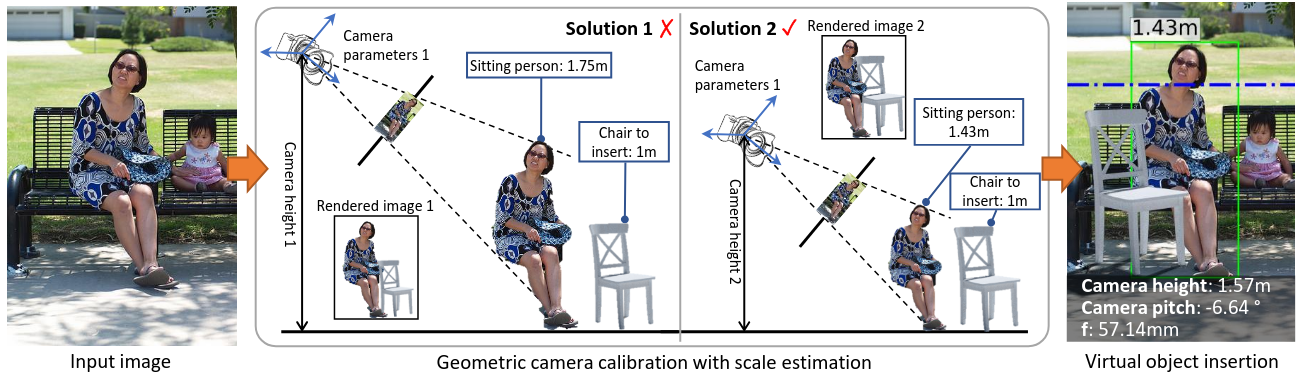
\includegraphics[width=0.7\textwidth]{ExampleObjectInsertion}
\end{center}
\caption{En metrología de vista única, se busca estimar la escala absoluta de la escena y, con ello, de los objetos detectados. De forma que no se observen diferentes soluciones en la estimación si los parámetros de la cámara, como la posición inicial, varían.
En la figura, sacada de~\cite{SingleViewMetrology}, se observa la imagen de entrada (izquierda), como podría varíar la estimación de escala (centro) y el resultado de ajustar los parámetros 3D para estimar (derecha).}
\label{fig:ExampleObjectInsertion}
\end{figure}

En la Figura~\ref{fig:Geometria} observamos la asociación entre los parámetros de la cámara, el objeto detectado, el modelado y estimación final.
Para ello, se utilizan los ángulos de la cámara, (yaw $\phi$, pitch $\theta$ y roll $\psi$), la longitud focal (f) y la altura de la cámara ($h_{cam}$). Para medir en el eje vertical, se busca 
la localización de la línea de horizonte ($v_0$) y centro de la imagen ($v_c$).
Con dichos párametros iniciales y el modelo de perspectiva, se pueden computar la relación entre los objetos en el plano 3D y el plano 2D con las siguientes ecuaciones~[\ref{eq:Vt}] y~[\ref{eq:Vb}]:
\begin{figure}[!ht]
\begin{center}
    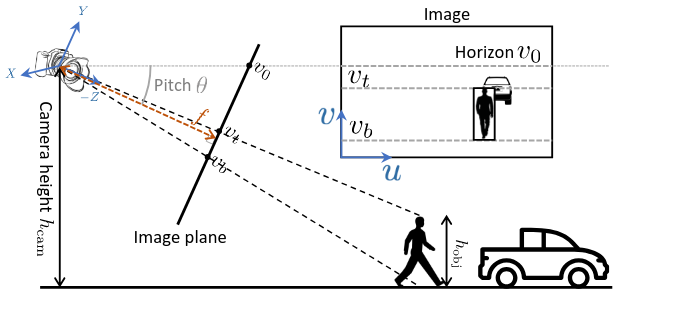
\includegraphics[width=0.5\textwidth]{Geometria}
\end{center}
\caption{Observamos el modelo de escena y el resultado obtenido (arriba), sacado de ~\cite{SingleViewMetrology}.}
\label{fig:Geometria}
\end{figure}
\begin{equation}
v_t = \frac{(fcos\phi+v_csin\phi)h_{obj} + (-fsin\phi + v_ccos\phi}{h_{obj}tan\phi + zcos\phi}
\label{eq:Vt}
\end{equation}
\begin{equation}
v_b = \frac{-fsin\phi z+v_ccos\phi z -fh_{cam}}{zcos\phi}
\label{eq:Vb}
\end{equation}
En la Figura~\ref{fig:Pipeline} podemos visualizar el flujo completo. Se utiliza Mast R-CNN~\cite{MaskRCNN}, un modelo de red neuronal convolucional, el cual se modifica para 
predecir la longitud focal a partir del campo de visión vertical. Adicionalmente, se utilizan cabezas adicionales para detectar el objeto en 
la imagen, el recuadro que lo delimita y puntos de interés. Cada paso tiene una función de pérdida específica. Se utiliza además una 
regularización con información apriori de que los humanos suelen medir $1.70\pm0.09m$ para personas y $1.59\pm0.21m$ para coches.
Una vez realizado la predicción, se hace un proceso de refinamiento. De forma iterativa, se observan los errores residuales y se predice la diferencia 
necesaria para cada parámetro estimado.
\begin{figure}[!ht]
\begin{center}
    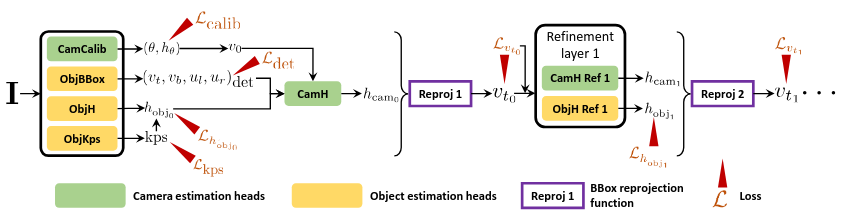
\includegraphics[width=0.7\textwidth]{Pipeline}
\end{center}
\caption{Observamos el flujo completo de la predicción. Donde tenemos cabezas de detección de los objetos (amarillo) y estimación de parámetros de
la cámara (verdes). Tenemos funciones de pérdidas distintas en cada parte (rojo) y funciones de proyección (lila).}
\label{fig:Pipeline}
\end{figure}
Para entrenar el modelo se hizo uso de múltiples conjunto de datos etiquetados. Para aprender a estimar los parámetros de la cámara, 
se hizo uso de la creación de los datos propuesto en~\cite{DeepSingleImageCalibration} (Calib). Para detectar y estimar el tamaño de los objetos se utiliza COCO-Scale, un dataset creado con el 
artículo proveniente de filtrar el original COCO~\cite{COCO}. Este último, tiene información de diferentes objetos, anotado con su recuadro e información adicional. 
Se filtra inicialmente usando Mask R-CNN~\cite{MaskRCNN} para detectar solamente las personas o coches. A continuación, buscamos ejemplos válidos, como los de la Figura~\ref{fig:Segmentacion}, en los cuáles 
se pueden observar en completo los humanos o coches para poder estimar el tamaño.
Una vez preparados los conjuntos de datos se entrena de forma secuencial, primero en Calib y luego en COCO-Scale. Algunos resultados 
se pueden observar en la Figura~\ref{fig:Resultados}.
\begin{figure}[!ht]
\begin{center}
    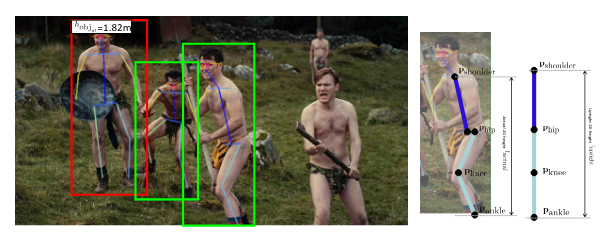
\includegraphics[width=0.6\textwidth]{Segmentacion}
\end{center}
\caption{Observamos ejemplos válidos de entrenamiento.}
\label{fig:Segmentacion}
\end{figure}

\begin{figure}[!ht]
\begin{center}
    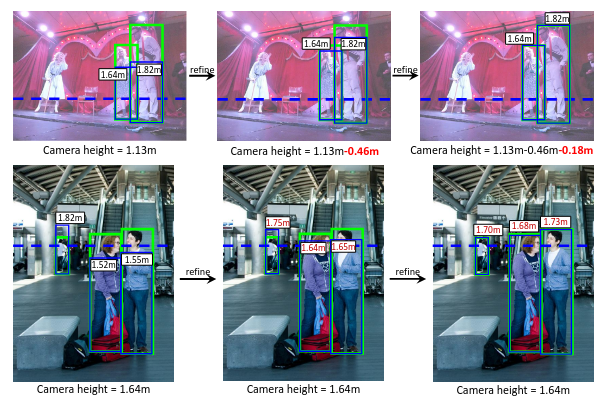
\includegraphics[width=0.6\textwidth]{Resultados}
\end{center}
\caption{Observamos una predicción inicial (izquierda) y el refinamiento (derecha).}
\label{fig:Resultados}
\end{figure}

\printbibliography
\end{document}
